\section{Results}

\begin{frame}{Results}
  \begin{figure}
    \centering
    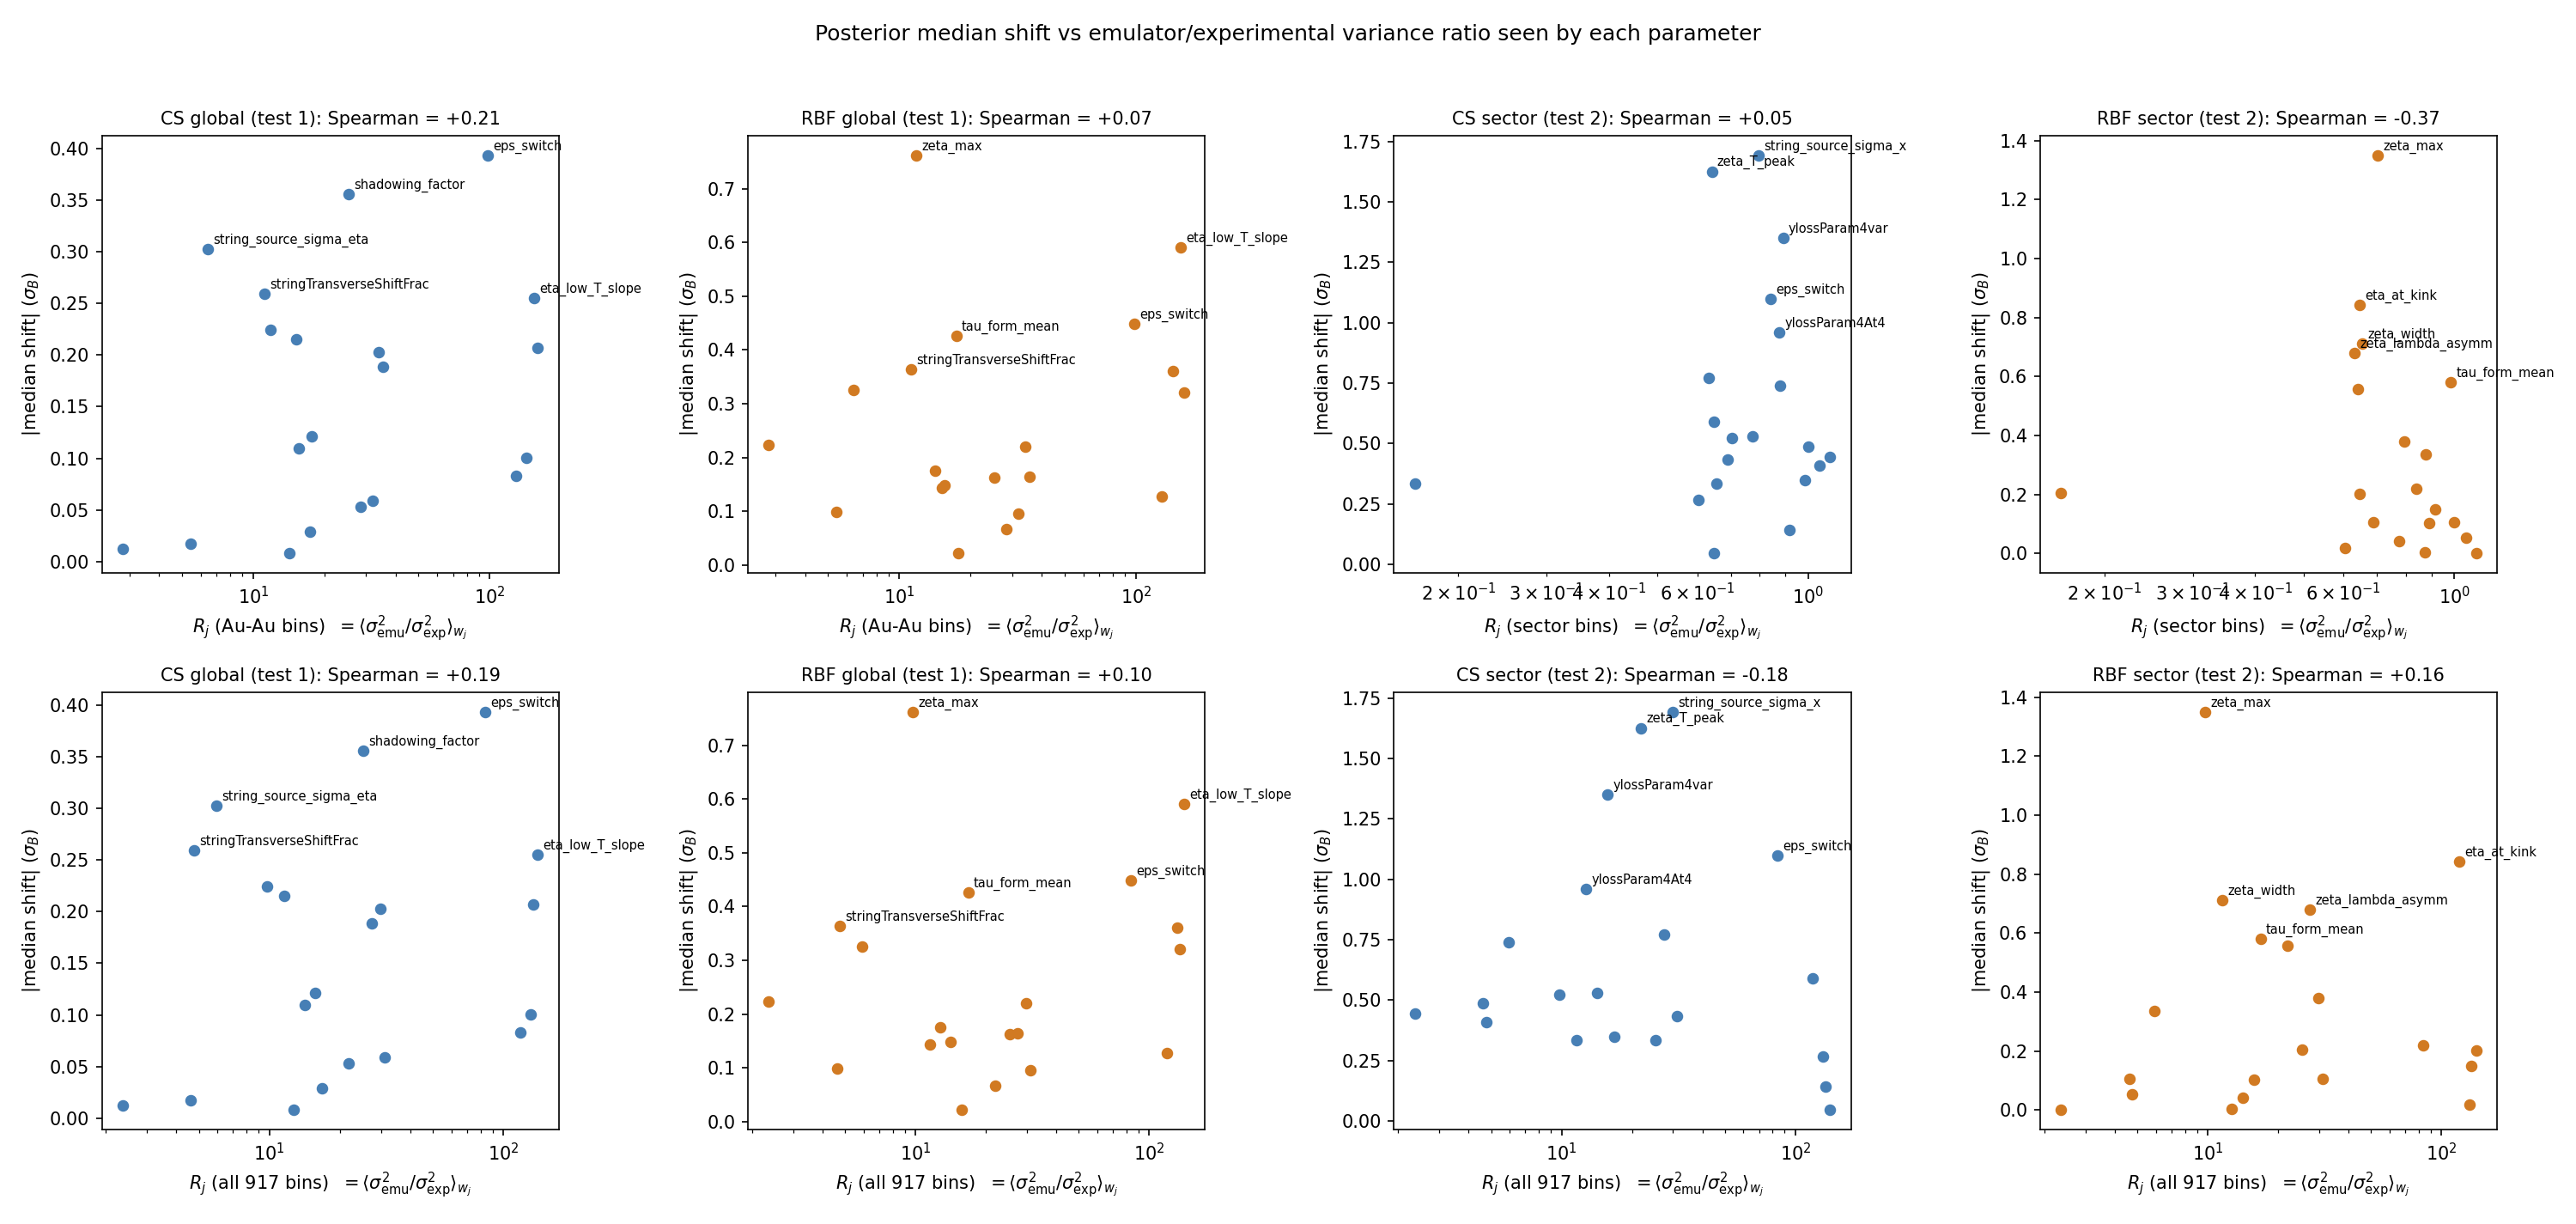
\includegraphics[width=\linewidth,height=0.67\textheight,keepaspectratio]{img/ng_shift_vs_cov_ratio.png}
    \caption{Posterior shifts for each parameter versus the weighted ratio of emulator to experimental variances, taken from the covariance diagonals. Global and sector correlation models probe how this uncertainty balance relates to changes in the inferred parameters.}
  \end{figure}
\end{frame}

\begin{frame}{Results}
  \begin{figure}
    \centering
    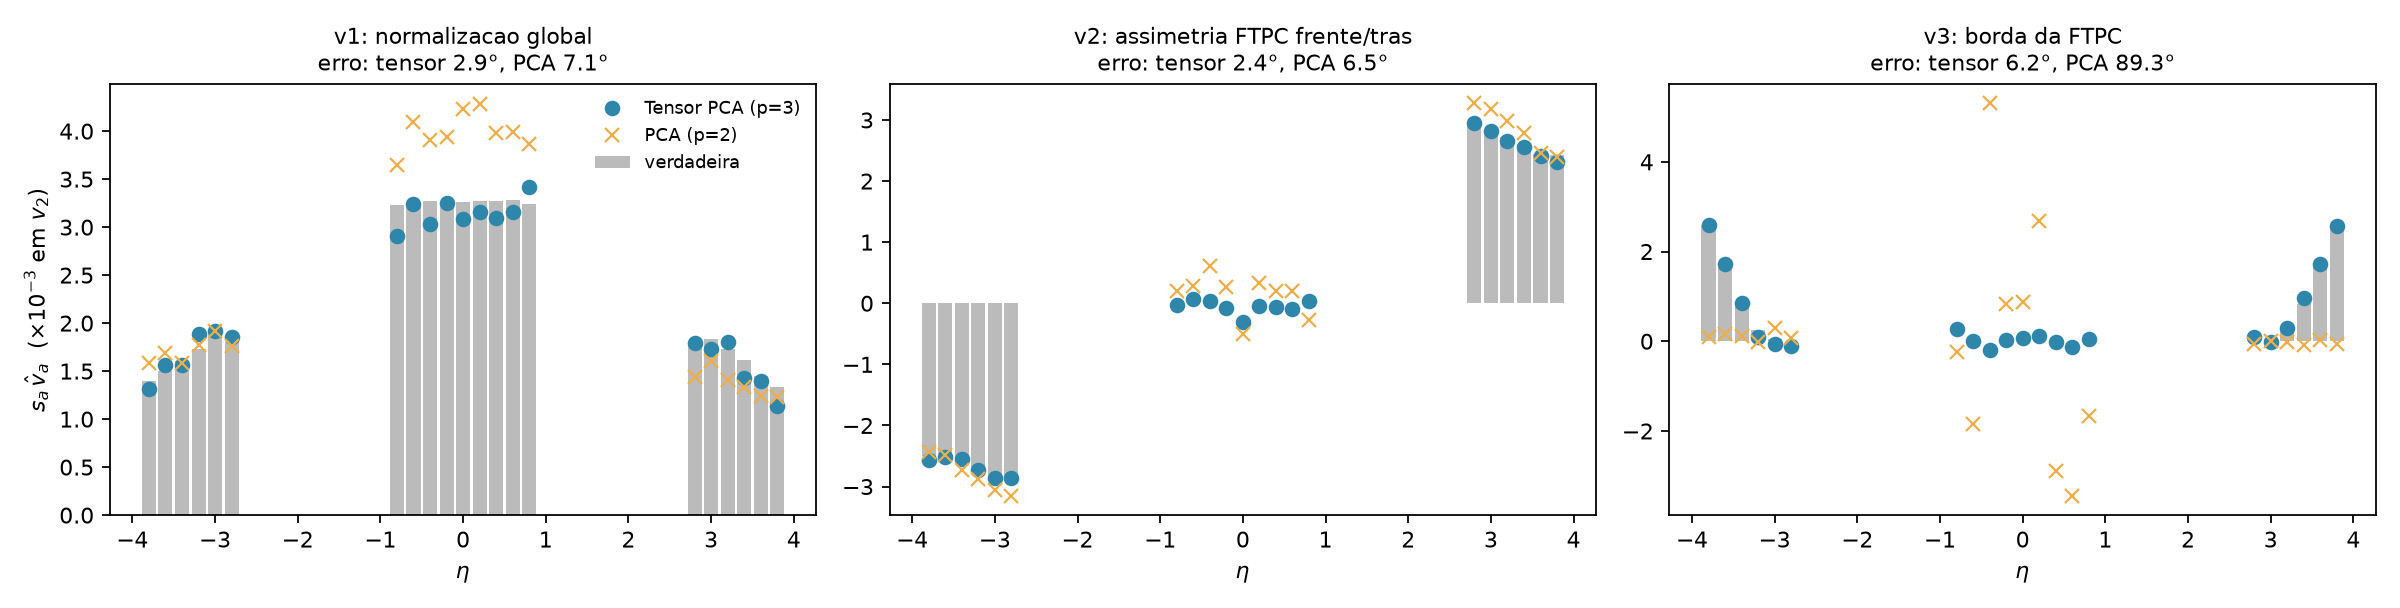
\includegraphics[width=\linewidth,height=0.64\textheight,keepaspectratio]{img/ng_sources_recovered_global.png}
    \caption{Tensor PCA and standard PCA reconstruct three underlying systematic-error sources. Tensor PCA follows the true source profiles more closely, especially the FTPC edge pattern that standard PCA struggles to recover.}
  \end{figure}
\end{frame}

\begin{frame}{Results}
  \begin{figure}
    \centering
    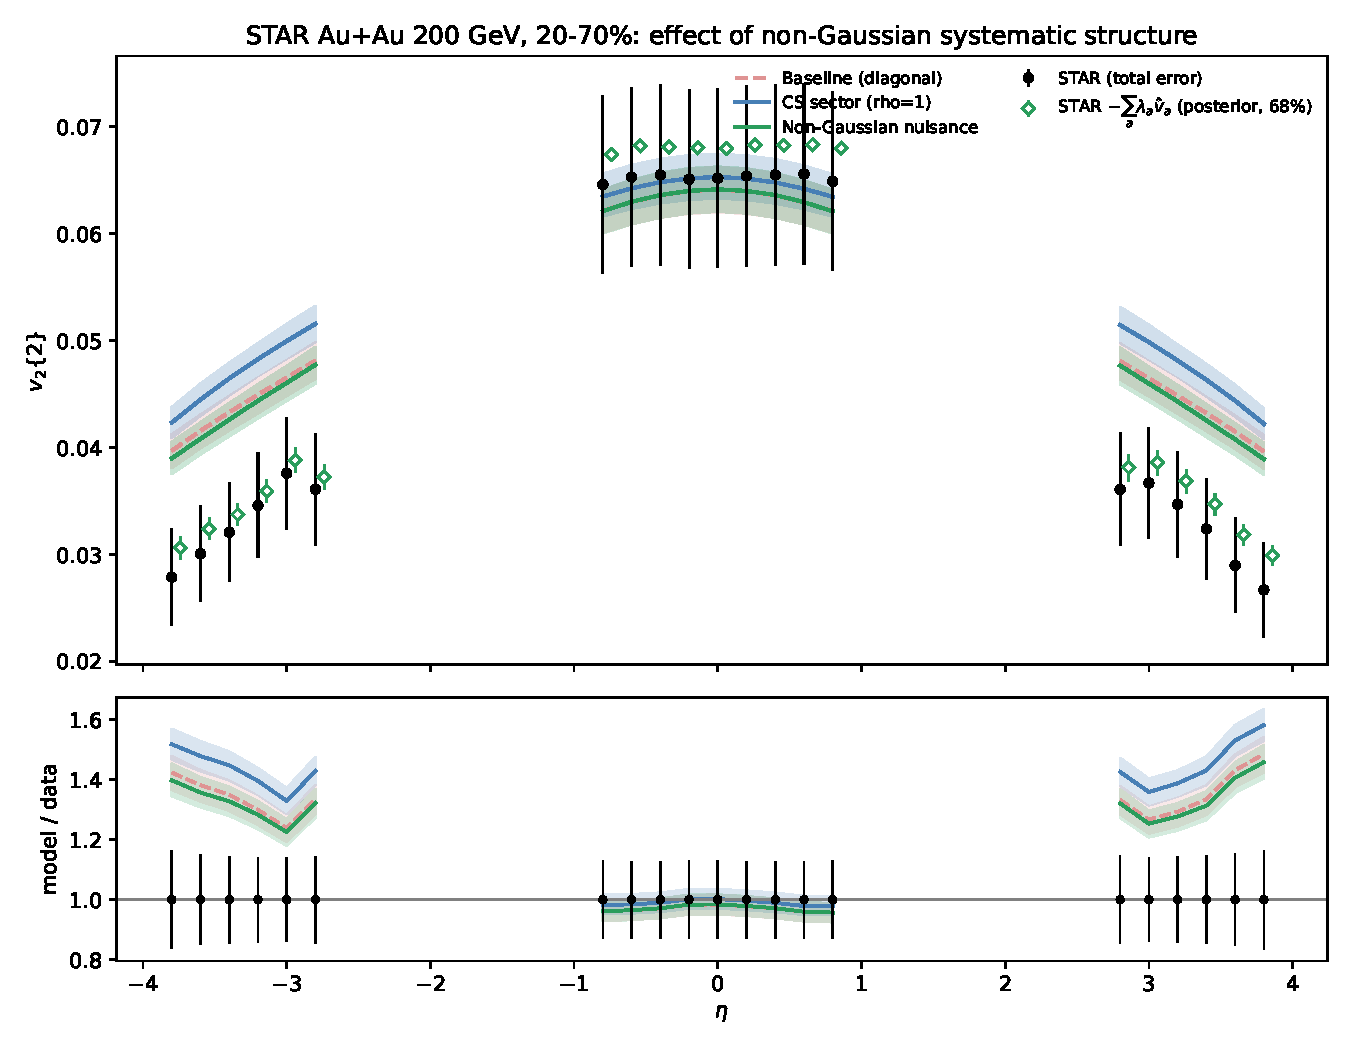
\includegraphics[width=\linewidth,height=0.67\textheight,keepaspectratio]{img/ng_star_v2_eta_3way.pdf}
    \caption{Posterior predictions for STAR $v_2\{2\}$ in Au--Au collisions at 200 GeV (20--70\% centrality). The diagonal baseline, sector CS model, and non-Gaussian nuisance model show how the treatment of systematic errors changes the inferred curves and their agreement with the data.}
  \end{figure}
\end{frame}
